\chapter{Reverse Image Search}

\label{chapter:ReverseImageSearch}

% ----------------

\section{Definition}
To better understand the definition and context of the Reverse Image Search problem, we first give the definition of two more general problems: Image Retrieval and Content-based Image Retrieval.

An image retrieval system is a computer system for browsing, searching and retrieving images from a large database of digital images. \cite{wiki:Image_retrieval} Examples of such a system are \textit{Google Image} \footnote{www.google.com} and \textit{Bing Image} \footnote{www.bing.com}, where the user writes a text query and have a list of images in return.

Content-based image retrieval (CBIR) is the application of computer vision techniques to the image retrieval problem. "Content-based" means that the search analyses the actual content of the image rather than the metadata such as keywords, tags, or descriptions associated with the image. \cite{wiki:Content-based_image_retrieval} An example of such a system is \textit{Google Image}, where the user can perform a search by image, either by URL or by uploading a file. If one submits an image of a cat, in return we will get images of visually similar cats, but not necessarily the exact same cat.

Reverse image search (RIS) is a content-based image retrieval (CBIR) query technique. The aim of a RIS system is to find the original of an image in a large image collection given a slightly modified version of it. An example of such a system is \textit{TinEye} \footnote{www.tineye.com}, where the user can submit an image and find out where this exact image appears on internet.

\subsection{Usage}
The main applications are listed in the FAQ \footnote{www.tineye.com/faq} of \textit{TinEye}.

\begin{itemize}
\item Find out where an image came from, or get more information about it
\item Identify duplicate images
\item Find a higher resolution version of an image
\item Locate web pages that make use of an image you have created
\item Discover modified or edited versions of an image
\item Show that the information provided with an image is false
\end{itemize}

Following are more specific use cases: A dating site can verify that a profile is authentic. An insurance company can detect fraud. Trademark offices can identify infringing trademarks. A museum can provide a mobile application on which the user can have additional details about a painting. A brand can replace QR codes and connect a printed catalog to an ecommerce platform.

\section{General framework}
Most approaches to Reverse Image Search share a similar pattern. It consists of: firstly, a way of representing an image, and secondly, a distance (or similarity) measure between two representations. As shown in figure \ref{fig:general_ris_framework}, RIS systems usually work in two phases: indexing and searching. During the indexing phase, representations of all the images in a collection are extracted and added to a database. The images are not necessarily stored in the database; this reduces its size. Afterward during the searching phase, a query image is presented to the system and its representation is extracted. A nearest neighbor search is then performed with the query representation, using the previously defined distance measure, to search for similar images in the database.

Reverse Image Search with large collections of images imposes two challenging constraints on the methods used. Firstly, for each image, only a small amount of data can be stored; secondly, queries must be very cheap to evaluate.

\begin{figure*}
	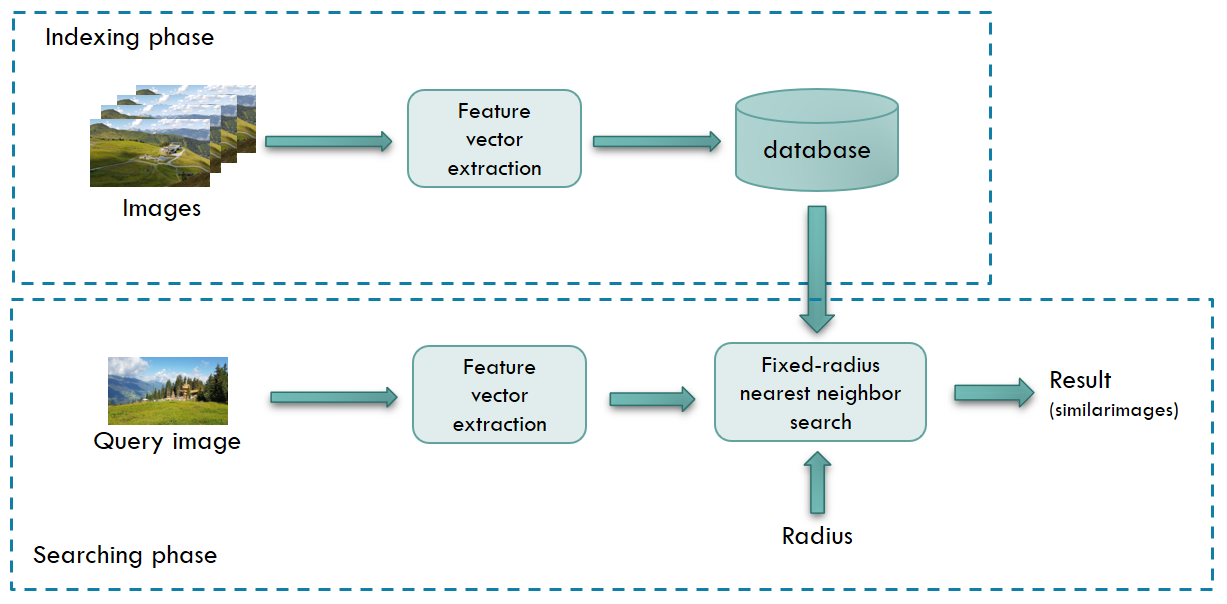
\includegraphics[width=\textwidth]{img/general_ris_framework.png}
	\caption{General framework for Reverse Image Search with fixed-radius nearest neighbor search.}
	\label{fig:general_ris_framework}
\end{figure*}

\subsection{Image representation}
The image representation is usually a $p$-dimensional vector of numerical features or a $q$-bit binary code. The feature vectors should be compact, in order to store millions of them in a database. Many algorithms are able to extract feature vectors from images based on color, texture, shape. We can classify features in two categories: low-level features, which are minor details of the image that are detected by simple algorithms: edges, corners, and so on, and high-level features, which carry more semantic and thus are better understandable by humans: objects, actions, and so on. High-level features are difficult to extract for computers because it is hard to understand the semantic of an image, this is currently an active research field. In the following part, we will describe some algorithms to extract low-level features from images.

A very simple approach is to compute the color histogram of an image. The image representation in this case is a vector of $N$-bins. If there is too much different colors in the image, it is possible to subsample the color space. To compare two histograms, we can use a distance based on correlation.

Color and Edge Directivity Descriptor (CEDD) \cite{chatzichristofis2008cedd} combines, in one histogram, color and texture information. The feature vector size is up to 54 bytes per image. The similarity between two CEDD histograms is measured with Tanimoto coefficient.

Scale-invariant Feature Transform (SIFT) \cite{lowe2004distinctive} extracts distinctive invariant features from images that can be used to perform reliable matching between different views of an object or scene. The features are invariant to image scale and rotation, and are shown to provide robust matching across a substantial range of affine distortion. SIFT detects key points in the image and compute small descriptor for each of them. The number of key points can vary and this is why a feature vector extracted with SIFT does not have a fixed length. To compare two images, their keypoints are matched by identifying their nearest neighbors, which can be very costly dependending on the number of keypoints.

The GIST descriptor was initially proposed in \cite{oliva2001modeling}. It is based on Gabor filters, which measure the orientations and spatial frequencies, and describes a scene with a set of perceptual dimensions (naturalness, openness, roughness, expansion, ruggedness). The GIST description is a feature vector of dimension 960, which can be compared with an Euclidean distance \cite{douze2009evaluation}.

\subsection{Distance}
To compare two image representations one has to choose a distance or similarity function. Depending on the representation many distances are possible.

\subsubsection{$p$-dimensional vectors}
If the image representation is a $p$-dimensional feature vector, following are distances or similarities between $x\in\mathbb{R}^{p}$ and $y\in\mathbb{R}^{p}$.

\textbf{Minkowski distance} is a generalization of Manhattan and Euclidean distances. Euclidean distance can be interpreted as the ordinary straight-line distance between two points in Euclidean space.

\[d_{minkowski}(x, y)=\left(\sum_{i=1}^n |x_i-y_i|^p\right)^{1/p}\]

When $p=1$, the Minkowski distance is equivalent to the Manhattan distance. When $p=2$, it is equivalent to the Euclidean distance. If the function is used to rank vectors according to their distance we can save time by not computing the nth root because this function is monotonically increasing.

\textbf{Cosine similarity} measures the cosine of the angle between two vectors. The cosine similarity is equal to 1 if the angle between vectors is 0. It is equal to 0 if the angle between vectors is $\pi/2$. 

\[s_{cosine}(x, y)=\cos{\theta{}(x, y)}=\frac{x\cdot{}y}{\norm{x}_2\norm{y}_2}\]

\[d_{cosine}(x, y)=\frac{\cos^{-1}s_{cosine}(x, y)}{\pi}\]

For example, the cosine similarity is used in information retrieval. In this field, documents are often represented as vectors containing the number of occurrences of terms. The cosine similarity is meaningful to measure the similarity of two documents regarding their subjects. In facts, what is important is not the number of time a term appears, but whether it appears or not.

Cosine similarity is related to Euclidean distance if the vectors are normalized to unit length.

\[\norm{x-y}^2=(x-y)\cdot{}(x-y)=x\cdot{x}+y\cdot{y}-2x\cdot{y}=\norm{x}^2+\norm{y}^2-2(\norm{x}^2\norm{y}^2\cos{\theta{(x, y)}})\]

Because $\norm{x}=\norm{y}=1$, we can conclude: 

\[\norm{x-y}^2=2(1-\cos{\theta{(x, y)}})\]

\subsubsection{Binary codes}
If the image representation is a $q$-bit binary code, following are distances or similarities between $a\in[0, 1]^{q}$ and $b\in[0, 1]^{q}$.

\textbf{Hamming distance} is the number of positions at which the bits are different. It measures the edit distance between two binary codes if the only allowed operation to transform the code is to flip a bit.

\[d_{hamming}(a, b) = \sum_{i=1}^{n} (a_i \oplus b_i)\]

On computers, this distance is straightforward to compute because it is the number of ones (population count) in the XOR of two binary codes. Since the population count and XOR are two basic operations in modern CPUs, the computation of Hamming distance is very efficient. Following is an implementation in C with two 64-bit binary codes using the POPCOUNT .

\lstset{language=C}
\begin{lstlisting}
int hamming_distance(uint64_t a, uint64_t b)
{
    return __builtin_popcountll(a ^ b);
}
\end{lstlisting}

\textbf{Simple Matching Coefficient} (SMC) is the number of matching bits divided by the length of the binary codes. It is useful when both a value of 0 and 1 for a bit carry equal information. SMC is used for comparing the similarity of two binary codes, to measure a distance one can use the Simple Matching Distance (SMD).

\[SMC=\frac{\text{number of matching bits}}{\text{number of bits}}=\frac{M_{00}+M_{11}}{M_{00}+M_{01}+M_{10}+M_{11}}\]

where:

\begin{description}
\item\textbf{$M_{00}$} is the number of positions where $a$ and $b$ both have a value of 0.
\item\textbf{$M_{01}$} is the number of positions where $a$ has a value of 0 whereas $b$ has a value of 1.
\item\textbf{$M_{10}$} is the number of positions where $a$ has a value of 1 whereas $b$ has a value of 0.
\item\textbf{$M_{11}$} is the number of positions where $a$ and $b$ both have a value of 1.
\end{description}

\[
\begin{split}
SMD & = 1 - SMC \\
    & = 1-\frac{M_{00}+M_{11}}{M_{00}+M_{01}+M_{10}+M_{11}} \\[3ex]
		& = \frac{M_{00}+M_{01}+M_{10}+M_{11}-M_{00}-M_{11}}{M_{00}+M_{01}+M_{10}+M_{11}} \\[3ex]
		& = \frac{M_{01}+M_{10}}{M_{00}+M_{01}+M_{10}+M_{11}}
\end{split}
\]

SMD is related to Hamming distance because $M_{01}+M_{10}$ is equal to the number of positions at which the bits are different, that is the Hamming distance.

\[d_{SMD}(a, b) = \frac{d_{hamming}(a, b)}{q}\]

\textbf{Jaccard Similarity Coefficient} is the number of positions where the two binary codes share a 1 divided by the number of positions where at least one binary codes has a value of 1. To measure a distance, one can use the Jaccard distance. The Jaccard Similarity Coefficient is very similar to the Simple Matching Coefficient, the only difference is that it does not take in account the positions where the two binary codes share a 0. It is useful for asymmetric binary data where a value of 0 and 1 for a bit does not carry equal information, for example a market basket data.

\[J = \frac{M_{11}}{M_{01}+M_{10}+M_{11}}\]

\begin{description}
\item\textbf{$M_{00}$} is the number of positions where $a$ and $b$ both have a value of 0.
\item\textbf{$M_{01}$} is the number of positions where $a$ has a value of 0 whereas $b$ has a value of 1.
\item\textbf{$M_{10}$} is the number of positions where $a$ has a value of 1 whereas $b$ has a value of 0.
\item\textbf{$M_{11}$} is the number of positions where $a$ and $b$ both have a value of 1.
\end{description}

\[d_{Jaccard}(a, b) = 1 - J = \frac{M_{01} + M_{10}}{M_{01}+M_{10}+M_{11}} = \frac{d_{hamming}(a, b)}{q - M_{00}}\]

It is possible to compute the term $M_{00}$ efficiently. It is the number of ones (population count) in $\neg(a \parallel b)$.

\subsection{Nearest Neighbor Search}
Nearest Neighbor Search (NNS) is the problem of finding in a database all the items whose distances to a query item are the smallest. Two variants are interesting for CBIR and RIS: k-nearest neighbors search and fixed-radius near neighbors.

K-nearest neighbors search aims to find the k nearest neighbors of a given query point. Usually the results are ordered by decreasing similarity (i.e. increasing distance). When applied to CBIR it is interesting in order to explore an image collection, because if the first results are not interesting, one can just look at the following results. 

Fixed-radius near neighbors aims to find all points that are within a radius of a given query point. Even if it is possible to sort the results according to the distance, the results should be considered as a set of unranked images. When applied to CBIR, this method is interesting for identifying content because only relevant images are returned, thus the result is composed of a varying number of images. The determination of an adequate radius, in accordance with the actual application, is critical. Information retrieval research has shown that precision and recall follow an inverse relationship \cite{datta2008image}. If the radius is too low, the precision is better at the expense of the recall, and vice versa. Depending on the application, one can want to favor precision, to authenticate content because there is fewer false-positives, or recall, to identify content because the user can deal with false positives.

Suppose our dataset is composed of $p$-dimensional feature vectors in a Euclidean space $D\equiv{\{x_i\}}_{i=1}^{n}$ where $x_i\in\mathbb{R}^{p}$. Let $z\in\mathbb{R}^{p}$ be a query feature vector, the one-nearest neighbor of the query $z$ is defined as:

\[KNN_{1}(z)=\argmin_{1 \leq i \leq n} \norm{z-x_i}^2\]

Let $r\in\mathbb{R}^+$ be a radius, the fixed-radius nearest neighbors of the query $z$ are defined as:

\[FRNN_{r}(z)=\{y \in D \;|\; \norm{y - z} \leq r\}\]

For $p$-dimensional feature vectors, there exist algorithms for exact nearest neighbor search such as the k-d tree, R-tree or MVP tree. But unfortunately, because of the curse of dimensionality, they are not efficient for high dimensional data (more than 20 dimensions). For this reason, Approximate Nearest Neighbor Search (ANNS) is gaining more interest because it allows for faster searching time with only small actual errors. In any case, we can refine a list of approximate nearest neighbors by pruning the items with the actual distance on the original features. The Locality Sensitive Hashing (LSH) framework is one approach to Approximate Nearest Neighbor Search and is detailed later in this part.